%!TEX root = thesis.tex

\chapter{A Brief and Opinionated Literature Survey}\label{chap:litsurvey}

The teleoperation systems are structurally interesting and equally challenging 
systems. This is especially true from a system theoretical point of view. As an example, 
if we just focus on the local and the remote devices that would be used for manipulation, 
we see that they are, whether linear or nonlinear, motion-control systems with well-studied 
properties. Hence, one can view the open-loop teleoperation as a system with a block 
diagonal structure. However, unlike the typical motion-control systems, these two disjoint systems must be stabilized 
simultaneously by the same controller, that is performing sufficiently in order to \enquote{fool} the user such that the user feels 
a force feedback as if s/he is actually operating at the remote medium. We need to emphasize that the 
delayed/undelayed local control loops can be seen as the entries of a structured central controller. Thus, there 
is no reason to distinguish control methods at this point.  

With this structure, the outputs of either of these subsystems become exogenous inputs of the other and these are regulated 
by the to-be-designed controller. Therefore, it is this controller that makes a teleoperation system perform 
adequately or, as in many cases, drive to instability.


For example, in the case of the so-called free-air motion (i.e. the remote device is free to roam in the remote site), the human force input 
to the local device and/or the position of the local device should\footnote{or better, that's what we believe today} 
be tracked by the remote device. In the case of a 
hard-contact of remote device with the environment, however, these inputs should be counteracted  if the force vector points into 
the obstacle. Hence, the force signal is simultaneously tracked for mimicking the user motion and  
is defied in case of a resisting force at the remote site. As if this is not challenging enough, 
when the user suddenly decides to release the local device, this resistance should die out as soon as possible, 
preventing a kickback. To sample the artificial nature of such behavior, consider a user who leans to a wall located at 
position $x_0\!\!\uparrow$, applying a horizontal force and then retreating after some time. It is not expected 
that the wall continues to push the user even after the user has the position $x<x_0$. This is not only unrealistic
but also misleading as it can be confused with a sticky surface as far as the immersion is concerned. There are many other 
scenarios that would further complicate the requirements but, in short, the user and the environment properties 
are time-varying and make it difficult to design a straightforward control law such that these and many other details are 
handled properly, and more importantly, simultaneously. 


With this short motivation, we can safely claim that looking at the overall system as a typical motion control 
system is not sufficient in terms of complexity (though necessary). In general, motion tracking specifications 
are a subset of the general performance requirements of the bilateral teleoperation systems. 

%\begin{rem}
%A similar line of reasoning has been given in \cite{buergerhogan1}. But for reasons that are 
%not known to us,  the authors chose to see the classical loop shaping as the sole servo control method. Moreover, modern 
%control theory offers a few options to avoid the obstacles that are given as impossibilities in their paper. Therefore, 
%we emphasize that the difference here is merely about the problem formulation and is not about the 
%limits of performance\footnote{We refer to the elegant book \cite{boydbarratt} for a detailed investigation of the 
%limits of performance.}. 
%\end{rem}


The inception of the bilateral teleoperation technology is often attributed to the work 
of Raymond Goertz in Argonne National Laboratories, \cite{goertz} (In \cite{basanezsuarez}, 
it's traced back to Nikola Tesla and, in \cite{sheridan89}, even some 16th century tools are accepted as precursors 
of the contemporary  teleoperation). The main motivation of Goertz' work (similarly later in Europe 
by Vertut \cite{vertutcoiffet}) was handling and manipulating nuclear material, thus the very 
first teleoperators were purely mechanical to cope with the hostile environment conditions. Though not much 
happened in terms of commercial product realizations, the concept of telemanipulation kept its appeal 
and a large body of research was reported until the 1980s. In that decade, with the help of the 
ever-increasing computational power and the popularity of Virtual Reality (VR), teleoperation 
technology received more attention for a possible use in the space-, underwater-, and medical-related 
tasks. Together with the advances in control theory and network theory (e.g. \cite{miyazaki,furuta}), 
a more systematic control methodology is adopted. Especially, stability analysis results that can be 
related to design guidelines (physical parameter bounds, bandwidth limitations etc.) were utilized
and limits of performance were explored. A particular phenomenon, namely the destabilizing effect 
of the delays in the teleoperation, lead the experts of the field to delve more into the systematic 
analysis tools and qualitative aspects of teleoperation. Especially, the use of the concepts; passivity, 
scattering transformations, and wave variables have become the standard methods of analysis and synthesis
(see, e.g., \cite{hannaford89,andersonspong,nieslotine}). We will start to summarize the advances from this 
point as this thesis is precisely built on top these systematic analysis and synthesis results gathered in 
the last two decades. However, the reader is refered to \cite{hokayemspong,burdea}, 
and \cite{sheridan89} for a more detailed overview including other practical aspects of teleoperation analysis and 
the hardware developments with a more historical perspective which we will omit here. 


As we keep on narrowing down our focus to the control theoretical parts of this challenging problem, we have to 
note that many parts of the bilateral teleoperation problem can be scrutinized under different frameworks. 
Hence, there is no shortage of techniques for which bilateral teleoperation problem is an ideal 
test case. In this plethora of methods, for example, the variation of human and environment properties give 
naturally rise to a robust or an adaptive control approach, the hard-contact problem can be analyzed under 
switched control systems, jump control systems or constrained linear systems etc. Thanks to these advances, 
as we will elaborate later, the main unsolved problem is not a methodolgical one but a motivational one. In
other words we are lacking a fundamental understanding of the problem not the solution methods in terms of 
what the requirements are and what a good device is if compared to another. Before we go into the 
details of the proposed methods of this thesis, let us sample a few important and successful approaches 
reported so far together with their shortcomings if any. We emphasize that the literature covered here is 
far from comprehensive and deliberately shaped with pragmatic intentions. Hence a large body of research is 
left out. This is certainly not due to their lack of thoroughness or else, but simply due to the irrelevance 
to the purpose of this chapter.


\begin{figure}%
%http://chat.stackexchange.com/transcript/message/4857161#4857161
\centering
\begin{tikzpicture}[scale=1,manstyle/.style={line width=4pt,line cap=round,line join=round}]
\node[rectangle,draw,minimum height=3cm,minimum width=3.8cm] at (0.5cm,0)     (a) {};
\node[rectangle,draw,minimum height=3cm,minimum width=3.8cm] at (1.5cm,1cm) (b) {};
\foreach \x in {north east,north west,south east,south west} \draw (a.\x) -- (b.\x);
\node[rectangle,draw,minimum height=3cm,minimum width=3.8cm] at (5.5cm,0)     (a) {};
\node[rectangle,draw,minimum height=3cm,minimum width=3.8cm] at (6.5cm,1cm) (b) {};
\foreach \x in {north east,north west,south east,south west} \draw (a.\x) -- (b.\x);
\node[fill,circle,inner sep=2.5pt,outer sep=1pt] at (-0.2mm,7.1mm) {};
\draw[manstyle] (0,0.5cm) -- ++(0,-1.2cm);
\draw[manstyle] (-1.5pt,0) -- ++(0,0.5cm) (1.2pt,1pt) --(0,5mm)--++(-45:4mm);
\draw[line width=1mm,fast cap-fast cap] (0.5cm,0.2cm) -- ++(0.5cm,0);
\begin{scope}[xshift=1.3cm,-stealth,black!20]
\draw (0,0,0) -- (0,0,1); \draw (0,0,0) -- (0,1,0);\draw (0,0,0) -- (1,0,0);
\end{scope}
\begin{scope}[xshift=4.7cm,-stealth,black!20]
\draw (0,0,0) -- (0,0,1); \draw (0,0,0) -- (0,1,0);\draw (0,0,0) -- (1,0,0);
\end{scope}
\begin{scope}[shift={(1.4cm,-0.2cm)}]
\draw (0,0) -- (0.9cm,0) (0.45,0) circle (1.5mm);
\path [fill=white] (0cm,0cm) rectangle (0.9cm,-0.16cm);%postaction={pattern=north west lines},
\draw[line width=1.5mm,round cap-round cap] (0.475cm,0.05cm) -- ++(110:7mm);
\draw[line width=1mm,round cap-round cap] (0.475cm,0.05cm) ++(110:6.3mm) --++ (220:5mm);
\end{scope}
\begin{scope}[shift={(5.4cm,-0.2cm)},cm={-1,0,0,1,(0,0)},transform shape]
\draw (0,0) -- (0.9cm,0) (0.45cm,0) circle (1.5mm);
\path [fill=white] (0cm,0cm) rectangle (0.9cm,-0.16cm);%postaction={pattern=north west lines},
\draw[line width=1.5mm,round cap-round cap] (0.475cm,0.05cm) -- ++(110:7mm);
\draw[line width=1mm,round cap-round cap] (0.475cm,0.05cm) ++(110:6.3mm) --++ (220:5mm);
\end{scope}
\draw[line width=1mm,fast cap-fast cap] (5.8cm,0.2cm) -- ++(0.5cm,0);
\begin{scope}[shift={(6.6cm,0.4cm)}]
\draw[thick]
\foreach \i in {1,2,...,10} {%
  [rotate=(\i-1)*36]  (0:2mm)  arc (0:12:2mm) -- (18:2.4mm)  arc (18:30:2.4mm) --  (36:2mm)
};
\node[circle,draw,inner sep=2pt,fill] (merkez) at (0,0) {};
\end{scope}
\begin{scope}[shift={(6.85cm,0cm)},scale=1.2]
\draw[thick]
\foreach \i in {1,2,...,10} {%
  [rotate=(\i-1)*36]  (0:2mm)  arc (0:12:2mm) -- (18:2.4mm)  arc (18:30:2.4mm) --  (36:2mm)
};
\node[circle,draw,inner sep=2pt,fill] (merkez) at (0,0) {};
\end{scope}
\begin{scope}[shift={(6.8cm,0.5cm)},scale=0.8]
\draw[fill] (0.5mm,0.5cm) rectangle (0.49cm,0.6cm);
\draw[fill,postaction={pattern=north west lines,pattern color=white}] (0.2cm,0.5cm) -- ++ (0,-0.4cm) -- ++ (-45:1mm) --++(45:1mm) --++ (0,0.4cm) --cycle;
\end{scope}

\end{tikzpicture}

\caption{General Teleoperation System}%
\label{fig:teleop}%
\end{figure}

\section{Modeling of Bilateral Teleoperation Systems}\label{sec:litchapmodeling}

The dominating modeling paradigm of bilateral teleoperation systems is the two-port network approach. Consider the following quote from 1989:
\begin{displayquote}[{\cite{hannaford89}}][.]
%In this paper, development of the analytical framework is complemented by modeling of an actual teleoperator system.
The modeling approach is to transform the teleoperation system model into an electrical circuit and simulate it using
SPICE, the electronic circuit simulation program developed at UC Berkeley
\end{displayquote}
%\end{mdframed}


As seen from Hannaford's motivation, the computer-based simulation tools are used extensively since then. Arguably
this is one of the main reasons why network based electrical circuit based modeling dominated the teleoperation literature. 
Reinforced with the circuit simulation tools, experts of the field started to construct analogies that go beyond
a mere mechanical-electrical system analogy. Arguably, the most prominent concept borrowed from these analogies is the two-port network 
view of the bilateral teleoperation systems. The reader is referred to \Cref{chap:apdxnetwork} for a short recap of network theory.
Today, the quoted convenience also applies to almost all physical systems i.e. one can simulate arbitrary models via many 
computational packages. Yet, it's a de facto standard to use the circuit modeling while the teleoperation devices are mostly 
mechanical. Hence, it's not clear whether the benefit of such an artificial step still exists. Once the system is represented 
by a mathematical model, as it is demonstrated in the later sections, the mechanical/electrical analogy is, roughly, an equivalence
based on the resulting model and works in the electrical$\to$mechanical direction too. Therefore, the 
circuit based modeling is merely a convention rather than a requirement.

\subsection{Two-port Modeling of Teleoperation Systems}

In the teleoperation context, if one uses the \enquote{load-source} analogy for the manipulated environment 
and the human, then the system models all the bilateral interaction between the load and the source 
ports (as in \Cref{fig:portrep}). This modeling view is quite powerful since the components are described via their input/output 
(or external) properties i.e. across variable/through variable relations (e.g. force/velocity, voltage/current etc.). Also, the non/linearity
properties of the components are not relevant at the outset if we are only interested in energy exchange which is the basis
of the so-called Time-Domain Passivity Methods \cite{hannafordryu} which we will mention later in this chapter. Thus, 
the user, the control system, the environment, the remote and local devices and communication delays are seen as 
$1$- and $2$-ports exchanging energy in time. Since the external behavior of the ports can be characterized completely by the 
current and the voltage drop across the terminals, it is indeed very convenient to model these components as 
interacting \enquote{black boxes} (See \Cref{fig:portrep}).

\begin{rem} We should emphasize here that in this context, the energy exchange is used as a gauge of a potentially unstable behavior. 
The motivation relies on the fact that in order to classify a system as an unstable one, the system should exhibit unstable
behavior at its port(s) and to exhibit such behavior additional energy is needed. Hence if all the components are incapable
of contributing energy in the loop, finite energy excitations will be eventually decay and the system would reach to its steady state
after a transient response\footnote{For the sake of brevity, eigenvalues on the imaginary axis or limit cycles are left out at this point.}. 
As one can directly identify, this is simply the rough sketch of the celebrated passivity theorem. Based 
on this argument, there is a recurring theme in the literature that a teleoperation system should be passive in order to have a stable 
interconnection. As we will mention later, this is due to the hypothesis that end terminations are also passive. However, in a few 
studies, this is mistakenly taken as a sufficient and necessary condition and hence creates quite some confusion for the non-experts 
of the field. Passivity is not an essential feature of the teleoperation systems but only a convenient shortcut for stability. We should 
iterate that the stability is the top-priority objective and does not require passivity by any means even if we do guarantee stability 
by rendering the sub-components passive. 
\end{rem}

\begin{figure}
\begin{subfigure}[b]{0.5\textwidth}
\centering
\begin{tikzpicture}[>=stealth,baseline=15mm,
every node/.style={draw,minimum size=1cm}]
\node (deltas) at (0,0) {$\Delta_l$};
\node[left=of deltas] (g) {$G$};
\node[left=of g] (deltal) {$\Delta_s$};
\tikzset{every node/.style={draw,circle,inner sep=1pt,fill=white}}
\foreach \y in {s,l}{
    \node at ({$(g)!0.5!(delta\y)$} |- {g.40}) (circ1\y){};
    \node at ({$(g)!0.5!(delta\y)$} |- {g.-40})(circ2\y){};
};
\draw (circ1l) -- (deltal.40) (circ2l) -- (deltal.-40)
(circ1s) -- (deltas.140) (circ2s) -- (deltas.-140);
\draw[->] (circ2s) -- (g.-40) (circ1s) -- (g.40);
\draw[->] (circ2l) -- (g.-140) (circ1l) -- (g.140);
\end{tikzpicture}
\caption{}
\label{fig:portrep}
\end{subfigure}%
\begin{subfigure}[b]{0.5\textwidth}
\centering
\begin{tikzpicture}[>=stealth,scale=0.5, transform shape]
\matrix (G) [draw,matrix of math nodes,inner sep=1mm,row sep=1mm,ampersand replacement=\&]{ G_{11} \& G_{12}\\ G_{21} \& G_{22}\\};
\matrix (delta) at (0,3) [outer sep=0,draw,matrix of math nodes,inner sep=0.5mm,ampersand replacement=\&]{\Delta_s \& \\ \& \Delta_l\\};
\draw[->] (G.160) -| ++ (-0.4,0.8) node[draw,circle,fill=white,inner sep=2,label={[inner sep=0]0:$\scriptstyle -$}] {} |- (delta.160);
\draw[->] (G.200) -| ++ (-0.7,0.6) node[draw,circle,fill=white,inner sep=2,label={[inner sep=0]0:$\scriptstyle -$}] {} |- (delta.200);
\draw[<-] (G.20) -| ++ (0.4,0.5) |- (delta.20);
\draw[<-] (G.-20) -| ++ (0.7,0.5) |- (delta.-20);
\end{tikzpicture}
\caption{}
\label{fig:nom_net}
\end{subfigure}
\caption{Two representations of a 2-port network.}
\end{figure}

Clearly, thanks to this modeling method, we don't even need to 
know exactly what $\Delta_l,\Delta_s$ blocks are, except their class (e.g. linear/nonlinear, time invariant/time varying etc.) to analyze 
the interconnection via $G$ and its port behavior.  Thus, the problem of modeling of the human arm or of the uncertain environment
is circumvented. However, with the same reasoning, passivity property does not distinguish particular systems as long as they are 
passive. That is to say, some of the crucial information is lost about these specific ports, we discard
any impedance or admittance relations shared by the port variables.

Energy based modeling is also the natural basis of bond-graphs. Bond-graphs, much like port representations, are graphical tools 
to model the dynamical systems via energy balancing between subcomponents (See \cite{gawthrop} for an introduction). In other words, 
the bond-graphs are built on top of the notion of bonds representing the instant energy or power exchange between nodes via edges 
drawn between them. Therefore, bond-graphs already presents a powerful framework for abstraction of the bilateral interaction between 
the local and the remote site. For a classical use of bond-graphs in impedance control, the reader is referred to the Hogan's trilogy 
(\cite{hogan:1,hogan:2,hogan:3}). There are also many studies with application focus, e.g., \cite{krishnaswamy} using hydraulic 
systems for bilateral teleoperation among many others. 



\subsection{Assumptions on the Local and Remote \enquote{Ports}}

As mentioned above, network theory offers a great opportunity for modeling the teleoperation systems, or better, avoiding 
the refined modeling. Still, to invoke the stability analysis and synthesis results of the network theory there is a need 
to further distinguish $\Delta_s,\Delta_l$ from the universum of $1$-ports. Otherwise there is not much we can conclude 
from such an interconnection, put differently, they can be any arbitrary models with arbitrary behavior set as long as they 
respect the port condition. This is obviously a crude approximation of the real physical interaction that teleoperation 
systems exhibit. 

In teleoperation and haptics literature, it is customary to assume the load and the source terminations as \enquote{passive}
mathematical operators (see \Cref{chap:apdxnetwork}). Starting with this hypothesis, the stability problem can be converted to 
a typical energy dissipation problem. 
Hence the view of the designer is tuned to watch for the energy sources and interaction between two distant media. This approach 
treats the human and the environment as passive $1$-port circuit elements with additional effort sources modeling the 
intentional force input to the system. The controller(s) act as the energy regulator preventing excess energy generation 
to avoid a possible instability. Moreover, as summarized in \Cref{chap:apdxnetwork} and in \Cref{chap:analysis}, one can use the 
network theory based conditions to assess the stability and performance conditions thanks to this hypothesis.

This brings us to the discussion of the justification of the assumption as it is generally not given in full generality in the
literature. If one scans through the literature about the passivity of human operators, it is the Hogan's paper \cite{hogan89}
that is almost universally cited. The striking detail is, however, that Hogan never claims that the human hand/arm is a passive
system. Instead he clearly shows that under certain conditions, human behavior is indistinguishable from that of a 
passive system: 
\begin{quote}
Thus, despite the fact that the
limb is actively controlled by neuro-muscular feedback, its apparent
stiffness is equivalent to that of a completely passive
system. In the light of Colgate's recent proof [3]\footnote{Reference 
\cite{colgatehogan88} of this thesis.} that an
apparently passive impedance is the necessary and sufficient
condition for a stable actively-controlled system to remain stable
on contact with an arbitrary passive environment, this
experimental result strongly suggests that neural feedback in the
human arm is carefully tuned to preserve stability under the
widest possible set of conditions.
\end{quote}
Moreover, the task that is given to human operators and analyzed afterwards, can be considered as a biased one because the success 
of the test is related to the passive behavior of the human. The task is, roughly speaking, holding a handle which is perturbed by 
random disturbances and trying to keep the handle still at a predefined position on the 2D plane. Hence, the task is simply to mimic 
a passive system. Had it been the case that the human would exhibit non-symmetric stiffness matrix, it would simply be a failure of 
the test subject (regardless of the physical limitations of the human arm in general). Note that this is a plausible situation for 
the rehabilitation tasks. The other possibility would then be that the test subject was unable to keep up with the changes, or using 
the control theory jargon, the bandwidth of the subject was lower than the required agility to perform the test adequately. The 
well-known phenomenon due to such behavior is the \enquote{pilot induced oscillations} in which the pilot of an aircraft, while trying 
to stabilize the aircraft, via overcorrection inputs, destabilizes the system due to many distinct reasons (the phase lag of the 
pilot, response time of the aircraft etc.). We refer to the interesting report \cite{mcruer} for a more detailed exposition. Also, 
if for some reason, the task at hand is to prevent the system to reach a steady state at a certain position and the perturbations are 
applied accordingly i.e., to create a virtual negative potential, the results obtained from the experiments would most probably differ 
from that of \cite{mussa85}. Thus, it's emphasized here that the passivity of the human is closely linked to the task requirements. 


\begin{rem}\label{rem:filament}
A particular detail should be clarified about the measurements taken in \cite{hogan89}. It is stated that: 
\begin{quote}
While normal human subjects held the handle of the manipulandum at a stable position
in the workspace, small perturbations were applied. Measurements
of the human's restoring force were made after the system
had returned to steady state following the perturbation but before
the onset of voluntary intervention by the subjects.
\end{quote}
Therefore, it is emphasized that only the involuntary response is taken into account during the measurements in order to
capture the natural properties human arm before the human correction intervenes. 
%Note that, this does not imply that the
%measurements treat the human arm as a bulk of flesh which might only be possible in case of an improbable amputation.
%In fact, in this setting, it is evident from the human restoring force that the arm muscles are preloaded and the arm is 
%cognitively locked at a certain position. 
%
%
%It is ththe voluntary input of the human is not included to the analysis, since the human necessarily puts in
%energy, at the very least, to move the local device. 
\end{rem}

We believe that it is unaviodable to introduce some concepts from the muscle physiology in order to put Hogan's 
argument into some mechanical engineering perspective. It is simply impossible for us to give a detailed analysis, 
however, mentioning the involved process via some mechanical analogies in order to relate the results of 
Hogan and Mussa-Ivaldi seems feasible. This would emphasize the reason why we think that the common inference 
from their experiments in the literature is not inline with the conclusions of these studies. We refer the reader 
to the physiology literature e.g., \cite{spudich,millman,offer,horowits,yildiz,geeves} and references therein for a full 
treatment. Hence, we will only give a rough picture about the apparent behavior. Nevertheless the point that we want 
to emphasize is, fortunately, not related to the inner workings of the human muscles.



%\begin{tikzpicture}
%\draw (-110:2) circle (1);
%\draw[double=gray,double distance=10,line cap=round] (0,0) -- (-95:1.5);
%\fill[red,rotate=30] (-5:0.9) -- ++(170:0.5) -- (-60:0.2) arc (-60:-200:0.2) --++(80:0.3) -- (117.5:0.9) arc (117.5:-5:0.9) -- cycle;
%\fill(0,0) circle (0.15);
%\fill[purple!45,rotate=30] [rounded corners=0.5pt] 
%(120:1) -- (120:0.5) arc(120:-7.5:0.5) -- (-7.5:1) arc (-7.5:0:1.2) 
%\foreach \x in {0,20,...,100}{-- (\x+2.5:1.2)   arc (\x+2.5:\x+10:1.2)  -- (\x+12.5:1)  arc (\x+13.5:\x+20:1.2)};
%\draw[dashdotted] (155:1.1) arc (155:15:1.1);
%\draw[fill] (-95:1.5) circle (0.15);
%
%\end{tikzpicture}
%\begin{figure}%
%\centering
%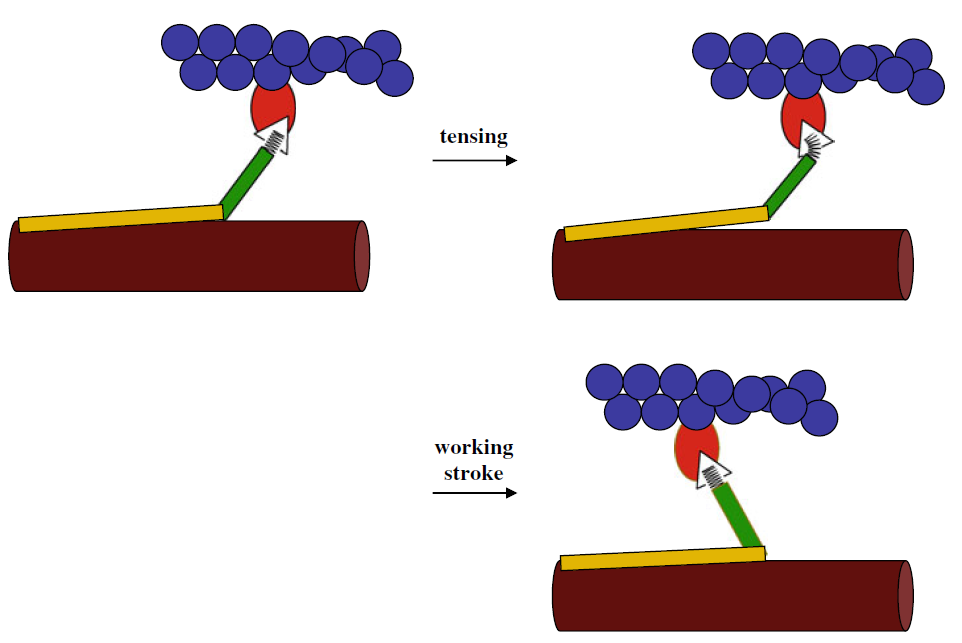
\includegraphics[width=0.7\columnwidth]{\impath/literature/muscleoffer}%
%\caption[Muscle activation mechanism]{Muscle activation mechanism (taken from \cite{offer}) Going to be drawn from scratch!!}%
%\label{fig:lit:muscle}%
%\end{figure}

\begin{figure}%
\centering%
\begin{tikzpicture}[transform shape, scale=0.5,decoration={zigzag,amplitude=1pt,segment length=1mm}]
\begin{scope}[]
\begin{scope}[]
\begin{scope}[rotate=90]
\draw[domain=0.6*pi/3:6.5*pi/3,
samples=50,draw=none,
mark=o*,
mark size=2mm,
mark options={fill=white},
mark indices={1,...,4,13,14,...,30,36,37,...,40,42,43,...,49}] plot[parametric] function{3*sin(t),0.1*sin(2*t)};
\filldraw[fill=white] (tpt-49) ++(10:2mm) arc (110:40:2mm) arc (-40:156:2mm) arc (65:5:2mm) ;
\fill (tpt-42) ++(150:2mm) arc (150:210:2mm) arc (330:30:2mm);
\end{scope}
\node[draw,anchor=west,shape=ellipse,ultra thick,minimum width=1cm] (a) at ([shift={(2mm,-3.5mm)}]tpt-42) (myo) {};
\node[draw,minimum height=5cm,minimum width=7mm] (actin) at ([shift={(2.5cm,-2mm)}]tpt-46) {};
\draw (myo.east) -- ($(myo.east)!0.5!(actin.north west)$) coordinate (a);
\draw[decorate] (a) -- ($(myo.east)!0.80!(actin.north west)$)coordinate (b);
\draw (b) --  (actin.north west);
\end{scope}
\begin{scope}[yshift=-7cm]
\begin{scope}[rotate=90]
\draw[domain=0.6*pi/3:6.5*pi/3,
samples=50,draw=none,
mark=o*,
mark size=2mm,
mark options={fill=white},
mark indices={1,...,4,13,14,...,30,36,37,...,40,42,43,...,49}] plot[parametric] function{3*sin(t),0.1*sin(2*t)};
\filldraw[fill=white] (tpt-49) ++(10:2mm) arc (110:40:2mm) arc (-40:156:2mm) arc (65:5:2mm) ;
\fill (tpt-42) ++(150:2mm) arc (150:210:2mm) arc (330:30:2mm);
\end{scope}
\node[draw,rotate=-20,anchor=west,shape=ellipse,ultra thick,minimum width=1cm] (a) at ([shift={(2mm,-3.5mm)}]tpt-42) (myo) {};
\node[draw,minimum height=5cm,minimum width=7mm] (actin) at ([shift={(2.5cm,-2mm)}]tpt-46) {};
\draw (myo.east) -- ($(myo.east)!0.5!(actin.north west)$) coordinate (a);
\draw[decorate] (a) -- ($(myo.east)!0.80!(actin.north west)$)coordinate (b);
\draw (b) --  (actin.north west);
\end{scope}
\end{scope}

\begin{scope}[xshift=7cm]
\begin{scope}[]
\begin{scope}[rotate=90]
\draw[domain=0.6*pi/3:6.5*pi/3,
samples=50,draw=none,
mark=o*,
mark size=2mm,
mark options={fill=white},
mark indices={1,...,4,13,14,...,30,36,37,...,40,42,43,...,49}] plot[parametric] function{3*sin(t),0.1*sin(2*t)};
\filldraw[fill=white] (tpt-49) ++(10:2mm) arc (110:40:2mm) arc (-40:156:2mm) arc (65:5:2mm) ;
\filldraw[fill=white] (tpt-42) ++(150:2mm) arc (150:210:2mm) arc (330:30:2mm);
\end{scope}
\node[draw,anchor=west,shape=ellipse,ultra thick,minimum width=1cm] (a) at ([shift={(7mm,-3.5mm)}]tpt-42) (myo) {};
\node[draw,minimum height=5cm,minimum width=7mm] (actin) at ([shift={(2.5cm,-2mm)}]tpt-46) {};
\draw (myo.east) -- ($(myo.east)!0.5!(actin.north west)$) coordinate (a);
\draw[decorate] (a) -- ($(myo.east)!0.80!(actin.north west)$)coordinate (b);
\draw (b) --  (actin.north west);
\end{scope}
\begin{scope}[yshift=-7cm]
\begin{scope}[rotate=90]
\draw[domain=0.6*pi/3:6.5*pi/3,
samples=50,draw=none,
mark=o*,
mark size=2mm,
mark options={fill=white},
mark indices={1,...,4,13,14,...,30,36,37,...,40,42,43,...,49}] plot[parametric] function{3*sin(t),0.1*sin(2*t)};
\filldraw[fill=white] (tpt-49) ++(10:2mm) arc (110:40:2mm) arc (-40:156:2mm) arc (65:5:2mm) ;
\filldraw[fill=white] (tpt-42) ++(150:2mm) arc (150:210:2mm) arc (330:30:2mm);
\end{scope}
\node[draw,rotate=-20,anchor=west,shape=ellipse,ultra thick,minimum width=1cm] (a) at ([shift={(7mm,-3.5mm)}]tpt-42) (myo) {};
\node[draw,minimum height=5cm,minimum width=7mm] (actin) at ([shift={(2.5cm,-2mm)}]tpt-46) {};
\draw (myo.east) -- ($(myo.east)!0.5!(actin.north west)$) coordinate (a);
\draw[decorate] (a) -- ($(myo.east)!0.80!(actin.north west)$)coordinate (b);
\draw (b) --  (actin.north west);
\end{scope}
\end{scope}
\end{tikzpicture}
\caption[Muscle activation mechanism]{Muscle activation mechanism (adapted from \cite{geeves})}%
\label{fig:lit:muscle}%
\end{figure}


The skeletal muscle activation takes place via a process described by the \emph{sliding filaments model}. The muscles 
consist of muscle fibers and muscle fibers are made up of \emph{myofibrils}. The myofibrils involve different types of thin 
and thick filaments, mainly of the type \emph{actin}, \emph{myosin} and \emph{titin} filaments. The myosin filaments involve 
extensions that can bind to the thin actin filaments. The relative motion of these filaments are produced due to these 
extensions via ATP hydrolysis. Moreover, these extensions stay connected or disconnected to actin filament unless more 
ATP is utilized. Hence, the muscle needs extra energy to relax which is the reason behind \enquote{\emph{rigor mortis}} 
and some types of the muscle spasms when this additional energy source can not be provided or ATP can not bind to the 
actin filament for some reason. Moreover, binding or detachment of these extensions is also regulated by the 
$\mathrm{Ca}^{++},\mathrm{Mg}^{++}$ concentration in the muscle cell and controlled, eventually, by motor neurons using yet another 
chemical trigger. 


Therefore, the individual muscle activation at the basic level is analogous to a clock escapement mechanism \cite{headrick} 
i.e. each time the lever arm pulls back a thread of the gear and the cycle repeats. The resulting relative motion is very much 
like a graphite coming out of a mechanical pencil when pressed from the eraser cap. Obviously, muscle behavior is not rachet-like 
but smooth. This is because each of these mechanism operate independently. Thus, at each time instant, different myosin extensions 
can be found at different phases of the cycle very much like a helical gear pair that are always in contact at one point. 
Using this analogy, ATP molecules are used to open and to close the pencil clutch made up of myosin extensions and actin filament 
is pushed forwards. Moreover, titin filaments can be thought as the connecting rod of the pencil from the cap to the clutch which 
is mostly responsible for the passive elasticity of the muscles. 

In summary, the muscles have varying non/backdrivable configurations. Moreover, we can lock our muscles in place
e.g., we can try to keep our arm at one position during drilling etc. to increase the precision. Then, the arm becomes
a stiff object with inherent stiffness of the connection rod (titin), pencil clutch (myosin actin), muscle tendons and
 various other involved processes resisting to the applied strain. 

Coming back to our original discussion, the stiffness of the arm that has been the subject of the experiments mentioned 
above is, again invoking the analogy, based on the closed clutch response of the arm. In other words, what is measured 
is a cumulative spring-like behavior of the arm that is actively controlled to be kept at a certain configuration. This 
is related to the \enquote{human's restoring force} given in \Cref{rem:filament}. 

Having a spring-like property naturally implies that the arm is passive. But the problem with this argument, as far as 
we understand, is that there is no reason to assume that the human arm exhibits a symmetric positive definite 
matrix at each time instant for an arbitrary trajectory. In fact, as shown clearly in \cite{mussa85}, the major eigenvector 
of the stiffness matrix varies both in terms of direction and magnitude. Therefore, it might be possible to extract energy 
from the human arm with some particular pathological trajectory. Just in the case of a frozen time analysis of a time-varying 
operator does not imply stability, the conclusion is only valid for postural analysis at a fixed configuration of the human arm 
but not for an arm trajectory. 

Therefore, it is our belief that the assumption of human arm being a passive operator is not an experimentally validated one. 
 


Since it is customary to include the passivity hypothesis in the literature, let us invoke it here too for the sake of the argument. 
The question of how, then, a human can possibly move anything while remaining passive is one that makes the whole story even more 
complicated. The voluntary input of the human is taken as an exogenous and state independent input to the system. Hence, the human 
cognitive input is an additional but independent force source acting on the handle together with the passive human arm immitance.


The reader would spot that this is not inline with Hogan's remark since the activation state in the muscle cells should be altered in 
order to apply force.In other words, we need to alter the stiffness matrix of the arm to be able to move but we have neither experience 
nor expertise to find out how. But, to the best of our knowledge, this is not given in any teleoperation study. In other words, the 
answer to the question of whether the human's restoring force would exhibit the same properties during the force exertion phase is 
not known to us. It has been also shown that muscle force is also related to the muscle tension-length properties \cite{eltit} 
which we have not considered in our analogy.

Therefore, we have to further separate the human force into two parts, namely, the active neuromuscular feedback force that keeps the 
human arm passive and the voluntary and cognitive force input applied to the system. How this is usually performed is not clear in the 
literature. To the best of our knowledge, this issue is considered (but still briefly) only in \cite[Sec. II.B]{kazeroonitsay} and 
references therein.


This ambiguity becomes much more important since the control oriented focus of this thesis necessitates that we concentrate on
worst cases rather than the experiments performed within the cognitive range of human operators. In other words, we are interested in
the cases where things go wrong due to many other various reasons, sampling disturbances, measurement noises, directionality etc. Therefore
it cannot be a satisfactory argument if stability depends on the user's neuromuscular feedback or simply user's stabilization capabilities. 
In order to use the bilateral teleoperation devices in real-life cases, stability should be addressed regardless of human actions. Hogan's 
findings are not sufficient for supporting the passivity assumption often found in the literature. 


In summary, the passivity of the human and the environment (virtual environment in haptics/virtual reality applications), is 
only plausible in certain cases which should be verified nevertheless in order to assume that the corresponding mathematical models 
are passive. Still, analysis and synthesis methods that invoke this assumption lead to many real-world implementations 
with varying degrees of realism. We argue that the success of these methods is due to the conservatism of the analysis/synthesis tools
and does not validate the passivity hypotheses on the respective models. Many frequency-domain methods, which assume LTI terminations
at both ends of the teleoperation network, are reported to achieve stable bilateral interaction in real setups. While impressive,
this shouldn't have been possible had the tests had not been exceedingly conservative since the real setups involve hard-contacts and 
time-varying systems. 


A compact version of the argument above is given by Yokokohji and Yoshikawa in \cite{yokokohjiyoshikawa}: 
\begin{quote}
Passivity of the system can be a
sufficient condition of stability only when the system interacts
passive environments. In the case of master-slave systems, if
we could assume that the operator and the environment are
passive systems, then the sufficient condition of stability is
that the master-slave system itself must be passive. Strictly
speaking, however, the operator is not passive because he/she
has muscles as the power source. Colgate et al. [21]\footnote{Reference 
\cite{colgatehogan88} of this thesis} mentioned
that even if the system has an active term, the system stability
is guaranteed unless the active term is in some way state dependent.
Obviously, the operator is passive when $\tau_{op}= 0$.
Therefore, we will give the following assumption about $\tau_{op}$:
\enquote{\emph{The operators input $\tau_{op}$ independent to the state of the
master-slave system. In other words, the operator does not
generate $\tau_{op}$ that will cause the system to be unstable.}}
Dudragne et al. [3] gave a similar assumption in order to use
the concept of passivity for stability distinction. The above
assumption seems tricky in a sense, but it is necessary to ensure
the system stability by the passivity.
\end{quote}

\noindent Finally, a supplementary remark is also given by Buerger and Hogan in \cite{buergerhogan1}: 
\begin{quote}
When passivity is used as a stability objective, the only assumption
made about the environment is that it, too, is passive.
This is likely sufficient to guarantee coupled stability with humans
(though, to date, it has not been conclusively proven that
human limbs are passive; see [29]\footnote{Reference \cite{hogan89} in this thesis} for an argument for treating
them as such). However, given the properties of human arms
described above, passivity is unnecessarily restrictive. Our experience
has shown that some controllers that are known to be
nonpassive are adequately stable in clinical rehabilitation tasks [26].
\end{quote}


We should mention here that Hogan's paper together with other identification experiments are extremely important for many
fields and needs no motivation. The discussion above only points out that the frequently reported inference that follows from 
his results, is not inline with the results. 

The idea of modeling the teleoperation as a two-port network seems to have multiple origins and we have no reference to 
point out to a common source. However, in general, the popularity of two-ports can be attributed to 
\cite{andersonspong,nieslotine,rajuphd,hannaford89,yokokohjiyoshikawa}. 



\subsection{Uncertain Models of Bilateral Teleoperation for Robustness Tests}\label{sec:lit:uncmodel}

Another possibility of modeling the human arm and its cognitive input is to define a reference position signal \enquote{filtered} by the 
human arm impedance\footnote{The term \emph{impedance} is used in a more general sense than its common usage to denote
LTI transfer functions such that no distinction is made between linear and nonlinear or time-invariant and time-varying 
operators.} e.g., \cite{leelee,kazeroonitsay}. Various studies pointed out that the identification experiments suggest a 
mass-spring-damper system pattern is evident in the frequency response data of the human arm recorded under various task 
performance similar to the one given in \cite{hogan89}. The general method is to instruct the human to perform a specific 
task and then perturb the hardware with certain predesigned disturbance signals such that the output can be evaluated to obtain 
a mathematical model. In the literature, the model structure is often set a priori to be a second order transfer function and 
the parameters are optimized to minimize the mismatch between the experimental and predicted response. It is also well-known 
that the human can change the inherent impedance of the arm during the task execution (see, e.g., \cite{tsujimorasso}). 
Therefore, the studies are performed in the ranges where it is safe to assume that the human arm characteristics are constant 
or constant up to negligible changes. 


The modeling is straightforward via uncertain mass-spring-damper system differential equation manipulations. Suppose the human arm
assumes the second order model: 
\[
M(\Delta_1)\ddot{x} + B(\Delta_2)\dot{x} + K(\Delta_3)x = F_h -F_m
\] 
where $F_h,F_m$ denote the human force and the force feedback inputs, respectively. Then choosing a multiplicative or additive uncertainty 
structure and via basic linear fractional transformations, the signal relations are converted to the interconnection shown in 
\Cref{fig:lit:figunc}. The arrows are deliberately left out as it's up to the designer to get different immitance models.
\begin{figure}%
\centering
\begin{tikzpicture}
\matrix[draw,matrix of math nodes] (m) {\Delta_1 &&\\&\Delta_2 &\\&&\Delta_3\\};
\node[below=1cm of m,draw,minimum size=2.0cm] (g) {$G_{nom}$};
\draw (g.155) -| ++(-1cm,1cm) |- (m.west);
\draw (g.25) -| ++(1cm,1cm) |- (m.east);
\draw (g.-155) -- ++(-1cm,0cm) (g.-25) -- ++ (1cm,0cm);
\end{tikzpicture}
\caption{Uncertain model representation by taking out the uncertainty blocks}%
\label{fig:lit:figunc}%
\end{figure}


Many studies have appeared in the literature regarding such modeling and the majority of these assume a 
mechanical model of order from two to five. Note that this is an assumption made a priori and only applies 
to the specific task performed by the human in the experiment from which the frequency response data is 
collected. The commonly utilized models can be found in \cite{kazeroonitsay,tsujigoto,kosuge,colgate1,speich,
fucavus,buergerhogan1,leungfa,husalculoewen,andrifour,laroche}. 
Obtaining these measurements are time-consuming and difficult to parameterize. For this reason, although
the results along this direction are scarce, they are, as in the passivity case, very valuable. 

The disadvantage of such parametrization of the human arm is contrasted with the passivity approach methods
invoking the argument of time-varying nature of the arm parameters. It is often rightfully argued that the 
uncertainty ranges in which the stiffness and damping (and partially inertial) coefficients change, are too 
large to be considered in the structured singular value based robustness tools. Moreover, many auxiliary 
effects such as the visual feedback, cognitive lag of the brain etc. are not considered in the identification 
experiments, but in the passivity approach all of these are lumped into a single port condition. Obviously, 
the main difficulty is to get a model (out of hypothetical insights, identification experiments etc.) which is
not required in the passivity approach.

The papers \cite{leelee,prekopiou} offer interesting alternatives for human modeling as they attempt to incorporate 
many of the aforementioned effects but the results are prospective and yet to be utilized. 



\section{Analysis}\label{sec:litchapanalysis}

The stability analysis is one of the major problems in designing stable yet high-performance teleoperation 
systems. It's often not feasible to manually tune some local controllers and make test subjects use it in order to verify the
design specifications. Moreover, relying only on the experiments can miss an important destabilizing scenario if the field 
experiments do not cover that particular case. Hence, an a priori certificate of stability is much sought after. The stability 
analysis can also give some guidelines about the parameter selection in the hardware design phase and can lead to minimized 
design iterations. Therefore, having a realistic stability test is essential in building these systems. 

Similar to the modeling section, the analysis in the literature extensively relies on network theory based results. In fact 
this is where the network theory stands out as a complete tool for analysis and synthesis of bilateral teleoperation systems
via the celebrated hypothesis that human and the environment models are passive.  

The common terminology for stability is somewhat different than that of the contemporary control theory as \emph{nominal stability} 
is used for the stability properties of isolated two disjoint media and when the interaction is setup between these two media the closed-loop 
stability problem is called \emph{coupled stability}. To the best of our knowledge, this terminology is introduced in 
\cite{colgatehogan88} hence we refer to this paper (or Colgate's thesis \cite{colgatephd}) for a more detailed motivation. 


It's also worth mentioning that the passivity and stability is used often interchangeably and also usually referred to the classical texts
\cite{haykin,mitra69,chen91} for the precise definitions. Hence, there is a little guesswork required to classify the stability definitions given in the
literature. The important distinguishing point is that the marginal stability is often accepted in the definition of stability results since
it arises frequently in lossless (hence passive) models where energy conservation is assumed. However, the analysis results often 
rely on such assumptions do not guarantee asymptotic interconnection stability but only lead to certain passivity 
properties of the interconnection (see \cite[Thm. 6.1]{khalil} and \cite[Sec. V]{lawrence} for the discussion on strict passivity).  

As given in \Cref{sec:litchapmodeling}, passivity property is crucial to many studies in the literature. The direct physical interpretation
of the abstract concepts gives even more appeal to such energy book-keeping methods. Another advantage of passivity methods is that 
the nonlinear counterparts of the results are also available in the literature and relatively easy to utilize. 

\begin{thm} The negative feedback connection of two passive systems is passive. The negative feedback connection of a passive system with
a strictly passive system is asymptotically stable.\end{thm}

Note that, this result is valid for both nonlinear and linear systems. Invoking the theorem twice on the teleoperation system allows us to conclude that,
under the passivity assumption of the human and the environment, if the two-port is  passive then the interconnection is passive. Moreover, if any of 
the involved operators is strictly passive the teleoperation system is asymptotically stable. 

\begin{figure}%
\centering
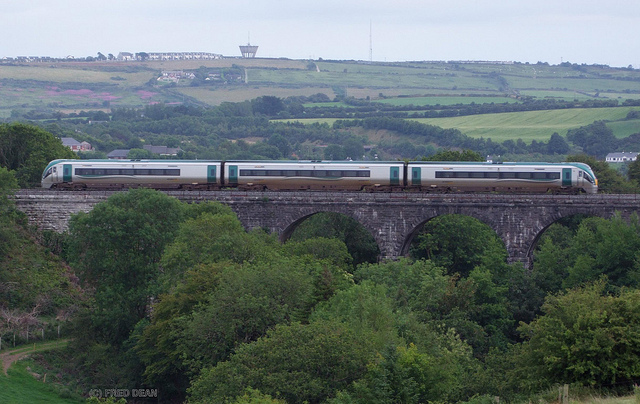
\includegraphics[width=0.6\columnwidth]{\impath/literature/train}%
\caption[A transparent two-port network with passive terminations]{A transparent two-port network with passive 
terminations. The actuation of the railcar is taken as state-independent input to the system. (Source: Fred Dean Jr., 
\href{http://www.flickr.com/photos/be216cd1/5971825854/}{[Flickr:Fred Dean Jnr]})}%
\label{fig:lit:train}%
\end{figure}


The passivity assumptions are not necessary for stability but only sufficient. Because there exist stable interconnections that involves nonpassive 
subsystems. In particular, the conservatism brought in by passivity theorem is arbitrarily high (especially in the nonlinear case). Facetious as it 
may seem, the test also takes into account the port terminations shown in \Cref{fig:lit:train} for a table-top joystick. We have to emphasize that
the three-carriage railcar with two cabs, is a valid, almost perfectly transparent two-port network. It's that conservative.


The major disadvantage of the passivity methods is that the procedure is focused almost only on the 
energy exchange. The performance specifications are very difficult to formulate and also difficult 
to integrate into the analysis and synthesis steps using only the inner product structure. As an 
example, the signals that are not port variables such as position errors, and nonlinear effects 
that are functions of these signals, can't be utilized easily in the performance specifications. 
Same difficulty arises in the normed space structures though much more can be achieved. Similarly,
peak-to-peak gain minimization methods are not mature enough to handle any practical system without 
excessive conservatism. 


Another disadvantage is that the power- or the energy-based analysis, due to the inner-product structure, can not distinguish the individual 
signal properties. Consider the ideal case where the human and the local device is pushing each other and cancelling each other's contribution. 
In this case the external or observable energy exchange based on the port variables is zero (negligible) which can not be distinguished from 
the case of not touching at all (a small motion on the device). 


When the network, human, and the environment models are assumed to be Linear Time Invariant (LTI), the frequency domain methods
allow us the analyze the teleoperation systems for stability and performance. The most common stabiliy analysis tool for such 
models is the Llewellyn's stability criteria (also often called absolute stability theorem or unconditional stability theorem). 
For linear networks, the following definitions seem to be used quite widely (modified from \cite{chen91}): 

\begin{define}[Potential Instability at $\iw_0$] A two-port network is said to be potentially unstable at $\iw_0$ on the real frequency, 
if there exist two passive one-port immitances that, when terminated at the ports, produce a persisting natural frequency at $\iw_0$.   
\end{define}

\begin{define}[Absolute Stability at $\iw_0$] A two-port network is said to be absolutely stable at $\iw_0$ on the real frequency, 
if it is not potentially unstable at $\iw_0$.   
\end{define}

Note that when the models are assumed to be LTI then absoulte stability theorem is an exact stability characterization. 

\subsection{Llewellyn Stability Criteria}\label{sec:llewellyn}
The well known conditions for stability of a two-port network, formulated in \cite{llewellyn,bolinder,rollett}, are recalled in \Cref{chap:apdxnetwork}.
As shown in \cite{rollett}, the conditions stated in \Cref{thm:apdx:llw} are invariant under immitance substitution. This result forms the 
basis for almost all passivity-based frequency domain bilateral teleoperation stability analysis approaches in the literature. 
We would also derive this theorem from an IQC perspective and show that it is actually the passivity counterpart of the 
of the $D$-scalings in the $\mu$-tools. This has been also derived in a scaled teleoperation context in \cite{poortenyokokohji}
using only SSV arguments. 

Thanks to the frequency domain formulation, it is possible  to rewrite the condition \eqref{eq:lit:llew3} as a fraction 
and see the problematic regions in which the fraction gets close to or crosses to the instability, together with one of the 
conditions given in \eqref{eq:lit:llew2}. 


\begin{figure}%
\centering
\begin{tikzpicture}[>=stealth]
\node[draw,minimum size=1cm] (h2) {$H_2$};
\node[draw,minimum size=1cm, above=1cm of h2] (h1) {$H_1$};
\node[draw,circle,inner sep=1mm,right= 1cm of h2]   (a1) {};
\node[draw,circle,inner sep=1mm,left= 1cm of h1,label={[inner sep=0]-60:$-$}] (a2) {};
\draw[->] (h1) -| (a1) node[right,midway] {$y_1$};
\draw[->] (h2) -| (a2) node[left,midway] {$y_2$};
\draw[->] (a1) -- (h2) node[above,midway] {$e_2$};
\draw[->] (a2) -- (h1) node[above,midway] {$e_1$};
\draw[<-] (a1) -- +(1cm,0) node[right] {$u_2$};
\draw[<-] (a2) -- +(-1cm,0) node[left] {$u_1$};
\end{tikzpicture}
\caption{Negative feedback interconnection}%
\label{fig:lit:passint}%
\end{figure}

\subsection{\texorpdfstring{$\mu$}{mu}-analysis}
As given in \Cref{sec:lit:uncmodel}, stability in the face of uncertainties can also be analyzed in the generalized plant framework 
of robust control. After rewriting the signal relations, the teleoperation system can be written as an uncertain interconnection as 
shown in \Cref{fig:lit:uncincgeneral}. In this setting, $G$ is the model of the nominal bilateral teleoperation system and $\Delta$ 
is a block diagonal collection of uncertainties, such as the human, the environment, delays, etc. Stability tests are based on structural 
hypotheses on the diagonal blocks of the operator $\Delta$ such as gain bounds or passivity. These properties should allow us to develop 
numerically verifiable conditions for the system $G$ that guarantee interconnection stability. This is intuitive because we have no access 
to the actual $\Delta$ and we can only describe its components by means of indirect properties. 

If the interconnection subsystems are represented in the scattering parameters, the $\mu$ test is precisely equivalent to the test of
Llewellyn's theorem and often called as Rollett's stability parameter. This is due to the well-known equivalence between the small-gain 
and passivity theorem \cite{desvid}. We have to note that the equivalence is stated in terms of the stability characterization. Otherwise, 
small-gain theorem requires a normed space structure whereas passivity theorem requires an inner product space structure, hence the 
applicability is relatively limited. This is also related to the fact that we need to work with power variables exclusively in the 
passivity framework and this is not always convenient if the performance specifications are related to other variables.

In the literature, this analysis method often follows the scattering transformations such that, the passivity assumption avoids the
explicit modeling and small-gain theorem allows to handle the delay problem via with bounded operators. A refinement can be found 
 in \cite{poortenyokokohji} as the authors utilize a direct $\mu$-analysis to reduce the conservatism, however rather remarkably, it's not
picked up by other studies and the analysis is mainly limited to small-gain conditions even in the linear cases. 


We can also directly take the uncertain modeling of the human and the environment and utilize $\mu$-analysis for the teleoperation
system. 



\begin{figure}%
\centering%
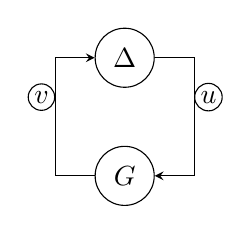
\begin{tikzpicture}[>=stealth]
\node[draw,minimum size=0.75cm] (plant) at (0,0) {$G$};
\node[draw,minimum size=0.75cm] (unc) at (0,1.5) {$\Delta$};
\draw[->] (plant.west) -| ++(-5mm,10mm) node[left] {$v$} |- (unc.west);
\draw[->] (unc.east)   -| ++(5mm,-5mm) node[right] {$u$} |- (plant.east);
\end{tikzpicture}
\caption{Uncertain Interconnection}%
\label{fig:lit:uncincgeneral}%
\end{figure}



\subsection{Modeling the Communication Delay}

Over the past two decades, it has been confirmed in various studies that, if present, the communication delays are a major 
source of instability (reports date back to 60's, e.g., \cite{sheridanferrell} and the references in \cite{andersonspong}).
Even when the delay duration $t$ is known and constant, delay operator can be shown to be nonpassive since
$e^{-st}$ is not positive real. Hence, when combined with the passivity framework, it violates the assumptions on the uncertain
operators. 


At end of the 80's and early 90's, two prominent studies (\cite{andersonspong,nieslotine}) proposed a direct handle to handle delay 
robustness problem using the scattering transformations. This notion is best explained, in our humble opinion, by loop transformations 
since the original articles refer to microwave and transmission line theories which use quite specialized terminology. One can also
find a slightly different system theoretical view of these transformations in \cite{colgate3}. If we restrict the discussion to LTI
operators\footnote{In the nonlinear case, it's a \emph{completion of square} argument to switch from the inner product structure to a 
norm structure provided that the signal space is suitable for such operation.}, the key concept of the scattering transformation
or the wave variables methods is mapping the closed right half plane to the closed unit disk via a special case of bijective M\"{o}bius 
(or linear fractional or bilinear) transformations: 
 
\begin{equation}
W:[0,\infty]\times i[-\infty,\infty] \mapsto \left\{ z\in\Complex \mid \abs{z} \leq 1 \right\}\, ,\, W(z) 
= \frac{z-1}{z+1}
\label{eq:lit:smith}
\end{equation}

One can directly verify that $1\mapsto 0,\infty\mapsto 1$ and $0\mapsto -1$ under $W$. Pictorially, the mapping is given in 
\Cref{fig:lit:smith} using a Smith chart which is located at the origin. Hence, positive real transfer matrices
become norm bounded by $1$ such that we can analyze the interconnection using the small-gain theorem.


Let us demonstrate a few properties of this transformation. First, this mapping can be shown with
a block diagram. Assume a proper positive real LTI SISO system $G(s)$ and let the input/output relation is given by $y=Gu$. Then, with a
standard manipulation, we obtain a feedback interconnection that leads to the mapping
\[
W(G(s)) = \frac{G(s)-1}{G(s)+1} = -1 + \frac{2G(s)}{G(s)+1} \Longrightarrow 
\begin{tikzpicture}[baseline=(g.center),scale=0.5,transform shape,every node/.style={draw,minimum size=1cm},every path/.style={->},>=stealth]
\node[draw] (g) at (0,0) {$G$};
\node[draw,left=1cm of g] (s1) {$\sqrt{2}$};
\node[draw,right=1cm of g] (s2) {$\sqrt{2}$};
\node[draw,circle, right=1cm of s2,minimum size=0,inner sep=3pt] (j) {};
\draw (s1) -- (g) node[midway,circle,fill=white,minimum size=2mm,inner sep=0] (f) {};
\draw ($(g)!0.5!(s2)$) |- ++(-1cm,-1cm) -| (f);
\draw (g) -- (s2);\draw (s2)--(j);\draw (j)--+(1cm,0);
\draw (s1) ++(-25mm,0) -- (s1);
\draw (s1) ++(-15mm,0) |- ([shift={(-1cm,1cm)}]j.center) -| (j);
\path (j)++(50:3mm) node[draw=none,minimum size=0,inner sep=3pt] {$-$};
\end{tikzpicture}
\]
Simply following the signal paths, we also see that the the input/output relation becomes
\[
\tilde{y}\coloneqq \sqrt{2}(-u + y) = W(G(s))\tilde{u}\coloneqq W(G(s))\sqrt{2}(u+y).
\]
Usually these variables are normalized with $\sqrt{2}$ at the outset. The distribution of $\sqrt{2}$ 
is a matter of convention and provides symmetry in the block diagrams. Also we have, 
\begin{align*}
(W\circ W)(G) &= \frac{-1}{G},\\
(W\circ W \circ W) (G) &= \frac{-1}{W(G)},\\
(W\circ W \circ W \circ W) (G) &= G\\
\end{align*}
which is nothing but the $90^\circ$ clock-wise rotations of the Riemann sphere about the axis parallel to the imaginary axis ($W$ is an element of 
M\"{o}bius group with $\circ$ operation). This is closely related to the stability parameter of Edwards and Sinsky (\cite{edsin}). 



\begin{figure}%
\centering
\begin{tikzpicture}[scale=0.6]
\begin{smithchart}[show origin,
axis background/.style={shading=eightball},
no marks,
grid=major,
axis equal,samples=150,
]
\foreach \t in {0,0.2,0.5,1}{
\addplot+[ultra thick,domain=-10:10] (\t,\x);
}

\end{smithchart}
\begin{scope}[shift={(8cm,0)}]
\begin{axis}[axis lines=middle,
grid=major,
no marks,
axis background/.style={right color=black!50,left color=white},
xmax=1.5,
%ytick=\empty,
every axis/.append style={
extra description/.code={
\node[xshift=-5mm] at (0,1) {Im$(z)$};
\node[xshift=-5mm] at (1,0.55) {Re$(z)$};
}}]
\foreach \x in {0,0.2,0.5,1}{
\addplot+[ultra thick] coordinates {(\x,-1.5) (\x,1.5)};
}
\end{axis}
\end{scope}
\end{tikzpicture}
\caption[Mapping the closed right half plane onto the unit disc.]%
{Mapping the closed right half plane onto the unit disc.}%
\label{fig:lit:smith}%
\end{figure}

Obviously once this transformation is introduced, there is a need for the \enquote{inverse} of $W$ on the operator that is seen
by the operator $G$ such that the loop equations remain unchanged, that is to say we have to introduce another transformation that undoes
$W$. The simplest way to obtain a mapping $\hat{W}$ is to follow the block diagram backwards as shown in 
\Cref{lit:syn:invscat}. A block diagram reduction step(or rotating three more times as shown above) shows that 
\[
\hat{W}(z) = -\frac{z+1}{z-1} = -\frac{1}{W(z)}
\]
The negative sign usually does not show up in the formulations in the literature because the passive interconnections 
require a sign change in the loop to indicate the \enquote{from} and \enquote{to} ports. A more detailed derivation
is given in \cite{colgate3}. Also note that a positive real transfer matrix, when negated, has its Nyquist curve 
confined in the close left half plane (anti-positive real) which is equivalent to a $180^\circ$ rotation. 
Thus, some care is needed for the book-keeping of the negative signs and seemingly the best practice
is to absorb the negative sign into $H$ at the outset and work with $-H$ afterwards. This makes the required
transformations identical. One can see that there are variants of this mapping, especially in wave variables 
definition, e.g., $\frac{z-b}{z+b}$ but for simplicity we take $b=1$ as it doesn't play any role in our 
presentation of the method. 


\begin{figure}%
\centering
\begin{tikzpicture}[scale=0.7,transform shape,every node/.style={draw,minimum size=1cm},every path/.style={->},>=stealth]
\node[draw] (g) at (0,0) {$G$};
\node[draw,left=1cm of g] (s1) {$\sqrt{2}$};
\node[draw,right=1cm of g] (s2) {$\sqrt{2}$};
\node[draw,circle, right=1cm of s2,minimum size=0,inner sep=3pt] (j) {};
\draw (s1) -- (g) node[midway,circle,fill=white,minimum size=2mm,inner sep=0] (f) {};
\draw ($(g)!0.5!(s2)$) |- ++(-1cm,-1cm) -| (f);
\draw (g) -- (s2);\draw (s2)--(j);
\draw (s1) ++(-15mm,0) |- ([shift={(-1cm,1.5cm)}]j.center) -| (j);
\path (j)++(50:3mm) node[draw=none,minimum size=0,inner sep=3pt] {$-$};
\node[draw] (h) at (0,-2cm) {$H$};
\node[draw,left=1cm of h] (is1) {$\frac{1}{\sqrt{2}}$};
\node[draw,right=1cm of h] (is2) {$\frac{1}{\sqrt{2}}$};
\node[draw,circle, right=1cm of is2,minimum size=0,inner sep=3pt] (j2) {};
\draw (j)-|++(1cm,-1cm)|-(j2);
\draw (h) -- (is1) node[midway,circle,fill=white,minimum size=2mm,inner sep=0] (f2) {};
\draw (is2) -- (h);\draw (j2)--(is2);
\draw ($(h)!0.5!(is2)$) |- ++(-1cm,-1cm) -| (f2);
\draw (is1) --++(-25mm,0) |- (s1);
\draw (is1) ++(-15mm,0) |- ([shift={(-1cm,-1.5cm)}]j2.center) -| (j2);
\path (f) ++(-70:5mm) node[draw=none] {$-$};
%\path (f2) ++(-70:5mm) node[draw=none] {$-$};
\end{tikzpicture}
\caption[Scattering transformation and its inverse.]{Scattering transformation and its inverse.}%
\label{lit:syn:invscat}%
\end{figure}


Under the mapping $W$, the Nyquist curve of $e^{-sT}$ (unit circle) is mapped onto the imaginary axis, 
hence unbounded, i.e.
\[
\frac{e^{-\iw T}-1}{e^{-\iw T}+1} = i\tan{\frac{\omega T}{2}}
\]
One can also obtain a similar qualitative result by seeing the unit circle $\mathbb{T}$ as the image of 
the imaginary axis under $W$: 
\[
W(\mathbb{T}) = (W\circ W)(i\widetilde{\omega} T) = \frac{1}{i\widetilde{\omega} T}
\]
We don't need to track the points individually as we are only interested in the domain and its image
under these transformations. 


This once again shows that delay uncertainty does not satisfy the norm constraint
$\|W(e^{-\iw t})\|_\infty \leq 1$ to invoke the small-gain theorem in the transformed coordinates. 
Had it been the case that the uncertainty was bounded by one, then it would have been possible to 
conclude stability directly in the passivity theorem anyhow. Thus, these transformations are not directly 
beneficial for analysis, however, following the cue from the previous mapping results, studies 
\cite{andersonspong} and \cite{nieslotine} 
made it possible to design controllers that takes into account this delay uncertainty. The resulting 
loop is stable regardless of delay period, hence they belong to the class of methods often distinguished
by \enquote{delay-independent} methods. According to the literature, these are the most common methods
applied in the face of delay uncertainty.

\subsubsection{Delay is Small-Gain}
Another possibility is to utilize the simple fact that the delay operator is gain-bounded and obtain the 
generalized plant by pulling out the uncertainty out of the loop. Obviously, this would be a very crude
characterization of the unit circle since as unit disk is used as the uncertainty instead. However, as 
we show later, wave variables/scattering transformations directly use this conservative formulation to 
model the delay in the stabilization of the loop.

A similar approach is reported in \cite{leungfa} using $\mu$-synthesis. By exploiting the
low frequency property of the operator $e^{-sT}-1$ and covering with a dynamic filter, the conservatism
is reduced. But the authors have omitted the uncertainty of the human and the environment. Therefore, 
their analysis is only valid for nominal teleoperation systems. Though, this can be extended to more 
general cases, we have to note that, they don't consider the human as \enquote{some impedance$+$state-independent 
force input} but as an finite-energy force input signal filtered through the human characteristics. 
Technically, this amounts to the common disturbance input-filtering often used in the $H_\infty$ design problems. 

 




\section{Synthesis}

Complementary to the analysis section, we cover a few popular controller structures among many others except the 
art of control engineering; manual PID tuning. 

\subsection{Two-, Three-, and Four-Channel Control Architectures}
In the teleoperation literature, the control laws are categorized in terms of how many measurement signals 
are sent over to the opposite medium during the teleoperation for control. The actual controller synthesis 
method is often not considered in this classification.  Hence, the naming \enquote{$n$-channel control}. The naming 
scheme can be better visualized as shown in \Cref{lit:syn:ela}. 


\subsubsection{Position-Postion and Position-Force Controllers}
The most basic control architecture among all is probably the PERR (position error) control in which the 
position of both local and the remote site devices are collected by the controller and control input is
produced.

Assume that the local and the remote device are at rest at position $x=0$ in the respective world coordinates. 
Also assume that the user moves the local device to position $x=\SI{10}{\centi\metre}$. What the control algorithm
should do is to measure the position difference and force each device accordingly to minimize the error. Hence, the
control law is of the form
\[
\pmatr{F_l\\F_r} = \pmatr{-1\\1} K_p(s) (x_l-x_r).
\]
where $F_r,F_l$ denote the control action at the local and the remote sites. $K(s)$ can be a constant or a SISO dynamical 
system or any other esoteric control law. One can perform the same with velocity signals (to comply with the passivity 
analysis) if available in noise-free measurements. Otherwise, position drift is unaviodable even with integral action. 

Typically, this control architecture would give a sluggish performance since there is no preference or priority in 
correcting the error signal on each side. Therefore, while the remote site is pulled forward to track the local device,
simultaneously, the local device is pushed back with the same force. This results with a feel similar to extending a 
damper, only in this case, it softens up according to the position error instead of travel velocity.

Another widely used, control architecture is the so-called Position-Force Controller. In this method the first channel 
in the PERR control structure is replaced with the remote site force input. Hence, local site device tracks the remote site 
encountered force while the remote site device tracks the position of the local site device. 
\[
\pmatr{F_l\\F_r} = \pmatr{K_f(s)F_{env} \\ K(s) (x_l-x_r)}.
\]
Clearly, the side-effect of PERR type control is avoided since the position and force errors are tracked independently 
in two seperate channels. But this brings in another tuning problem: If the position control gain dominates, the force tracking 
behaves aggresively in the hard contact case due to the overuse of control action to drive the remote device into the obstacle
and generally results with kickback or the local device. Conversely, domination of the force gain results with chattering of 
the remote device on the obstacle due to the discontinuous nature of the force reference signal if the user touches the handle 
with just softly enough to sustain an oscillation. Therefore, not only the gains of the individual channels are hard to tune, but
also relative magnitudes of the gains makes the tuning more tedious. In practice, 

\subsubsection{Force-Force+PERR}

To increase the bandwidth and to reduce the side-effects of aforementioned methods, a feedforward controller is added to the 
position-force control architecture. 
\[
\pmatr{F_l\\F_r} = \pmatr{K_{f1}(s)F_{env} \\ K(s) (x_l-x_r)+K_{f2}(s)F_{hum}}.
\]
Hence, the name a three-channel controller. This has been introduced in \cite{hashzaad1999} and also analyzed in \cite{naerumhannaford}.

\subsubsection{Lawrence Control Architecture}

In \cite{lawrence}, a general control scheme is proposed (later extended by \cite{salcudeanzhu,hzaadsalcu2}). In this architecture, 
also the remaining channel of remote position is sent over to the local site, completing the number of channels transmitted to four.
The individual controller blocks and the resulting overall block diagram is shown in \Cref{lit:syn:ela}.  

\begin{figure}%
\centering
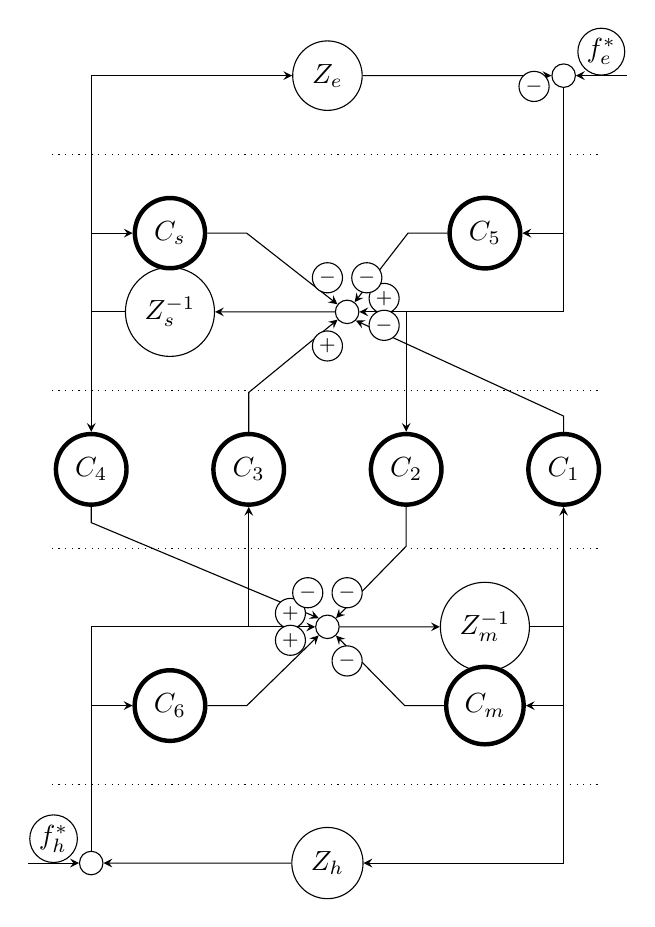
\begin{tikzpicture}[
imp/.style={draw,inner sep=4pt},
impc/.style={draw,inner sep=4pt,ultra thick},
junc/.style={draw,circle,inner sep=3pt},>=stealth]
\begin{scope}[xshift=-3cm]
\node[impc] (c4) at (0,0) {$C_4$};
\node[impc] (c3) at (2cm,0cm) {$C_3$};
\node[impc] (c2) at (4cm,0cm) {$C_2$};
\node[impc] (c1) at (6cm,0cm) {$C_1$};

\node[imp] (zinvs) at (1cm,2cm) {$Z_s^{-1}$};
\node[impc] (cs) at (1cm,3cm) {$C_s$};
\node[impc] (c5) at (5cm,3cm) {$C_5$};
\node[imp] (ze) at (3cm,5cm) {$Z_e$};

\node[imp] (zinvm) at (5cm,-2cm) {$Z_m^{-1}$};
\node[impc] (cm) at (5cm,-3cm) {$C_m$};
\node[impc] (c6) at (1cm,-3cm) {$C_6$};
\node[imp] (zh) at (3cm,-5cm) {$Z_h$};
\end{scope}
\foreach \x in {1,4}{
\draw[dotted] (-3.5cm,\x) --(3.5cm,\x) (-3.5cm,-\x) --(3.5cm,-\x);
}
\foreach \x[count=\xi] in {(0.25,2),(3,5),(0,-2),(-3,-5)}{
\node[junc] (j\xi) at \x {};
}
\draw[->] (zinvs.west) -| (c4);
\draw[->] (zinvs.east -| c4) |- (cs.west);
\draw[->] (cs-|c4) |- (ze);
\draw[->] (ze) -- (j2);
\draw[->] (j2) |- (c5);
\draw[->] (j2 |- c5) |- (j1);
\draw[->] ({{j2 |- j1}}-| c2) -- (c2.north);
\draw[->] (c1.north) -- ++(0,2mm) --(j1.-45);
\draw[->] (cs.east) -- ++(5mm,0) --(j1);
\draw[->] (j1) -- (zinvs);
\draw[->] (c5.west) -- ++(-5mm,0) --(j1);
\draw[->] (c3.north) -- ++(0,5mm) --(j1);

\draw[->] (zinvm.east) -| (c1);
\draw[->] (zinvm.east -| c1) |- (cm.east);
\draw[->] (cm-|c1) |- (zh);
\draw[->] (zh) -- (j4);
\draw[->] (j4) |- (c6);
\draw[->] (j4 |- c6) |- (j3);
\draw[->] ({{j4 |- j3}}-| c3) -- (c3.south);

\draw[->] (c4.south) -- ++(0,-2mm) --(j3.135);
\draw[->] (cm.west) -- ++(-5mm,0) --(j3);
\draw[->] (j3) -- (zinvm);
\draw[->] (c6.east) -- ++(5mm,0) -- (j3);
\draw[->] (c2.south) -- ++(0,-5mm) --(j3);

\draw[<-] (j2) -- ++(8mm,0) node[midway,above] {$f^*_e$}; 
\draw[<-] (j4) -- ++(-8mm,0) node[midway,above] {$f^*_h$};

\path (j2) ++(200:4mm) node {$\scriptstyle-$};
\foreach \x/\y in {20/+,60/-,120/-,240/+,-20/-}{
\draw (j1) ++(\x:5mm)node   {$\scriptstyle\y$};
}
\foreach \x/\y in {160/+,120/-,60/-,-60/-,200/+}{
\draw (j3) ++(\x:5mm)node   {$\scriptstyle\y$};
}
\end{tikzpicture}
\caption[Extended Lawrence Architecture]{Extended Lawrence Architecture, adapted from \cite{hashzaad1999}. 
Starred signals are the exogenous force inputs by the human/environment}%
\label{lit:syn:ela}%
\end{figure}


Instead of such classification, one can directly start with a MIMO control structure while keeping the control problem formulation fixed. For this purpose, consider the 
control mapping $K:\Real^{n_1}\times\Real^{n_2}\times\Real^3\times\Real^3\to \Real^{m_1}\times\Real^{m_2}$ from the 
measurements to the local and remote control actions via 
\begin{equation}
\pmatr{F_l\\F_r} = K \pmatr{x_l\\x_r\\F_{hum}\\F_{env}} 
\vcentcolon = 
\tikz[baseline=(m.center),
every left delimiter/.style={xshift=1ex},%tighter delimiter spacing
every right delimiter/.style={xshift=-1ex}]
{\matrix[matrix of math nodes,
ampersand replacement=\&,
left delimiter={[},
right delimiter={]},
nodes={minimum width=1cm}
](m){
-C_m \& |[fill=gray]| C_4 \& C_5 \& |[fill=gray]|-C_2\\ 
|[fill=gray]|C_1  \& C_s \& |[fill=gray]|C_3 \& -C_6\\
};
}
\pmatr{x_l\\x_r\\F_{hum}\\F_{env}}
\label{eq:lit:MIMOcont}
\end{equation}
where $n_1,n_2$ denote the number position measurements and $m_1,m_2$ denote the actuation inputs with overactuated 
robotic manipulators in mind. The grayed entries are the control subcomponents that works with the variables sent over 
the network. If we recap the architectures above with this notation, they can be represented as
\[
K = \bmatr{
-k &k&0&0\\
k&-k&0&0
}\pmatr{x_l\\x_r\\F_{hum}\\F_{env}},
\]
\[
K = \bmatr{
0&0&0&k_f\\
k&-k&0&0
}\pmatr{x_l\\x_r\\F_{hum}\\F_{env}},
\]
\[
K = \bmatr{
0&0&0&k_{f1}\\
k&-k&0&k_{f2}
}\pmatr{x_l\\x_r\\F_{hum}\\F_{env}}
\]
respectively. Each of the lower case $k_i$ represents some constant or dynamic controller. Obviously, one can 
generate many more architectures populating different entries and the zero blocks. 


\subsection{Wave Variable-Scattering Transformation Control for delays}

We have discussed the transformation from a passive interconnection to small-gain interconnection however
we have assumed that the interconnection did not involve any communication delays. When the delays are 
introduced to the loop as depicted in \Cref{lit:syn:delinc}, the transformations actually shift the stability problem from
one domain to another. In other words, the transformations make the delay operators unbounded-gain as we have showed previously. 
Therefore, interconnection of passive and small-gain operators avoids to be handled by neither small-gain nor passivity theorems. 
Hence, we are left with the only option to modify the system. This technique has dominated the literature thanks to 
\cite{andersonspong,nieslotine, nieslotine2}. 

%
%\begin{figure}%
%\centering
%\begin{tikzpicture}[%scale=0.8,
%transform shape,
%every node/.style={draw,minimum size=1cm},
%every path/.style={->},>=stealth]
%\node[draw] (g) at (0,0) {$G$};
%\node[draw] (h) at (0,-2cm) {$H$};
%\node[draw] (d1) at (2cm,-1cm) {$e^{-sT}$};
%\node[draw] (d2) at (-2cm,-1cm) {$e^{-sT}$};
%\draw (h) -| (d2);\draw (d2) |- (g);
%\draw (g) -| (d1);\draw (d1) |- (h);
%\end{tikzpicture}
%\caption[A delayed interconnection]{A delayed interconnection (Negative feedback sign is included in $H$)}%
%\label{lit:syn:delinc}%
%\end{figure}

\begin{figure}%
\centering
\begin{tikzpicture}[%scale=0.7,
>=stealth,
]
\begin{scope}[transform shape,
every node/.style={draw,minimum size=1cm},
every path/.style={->},
shift={(-7cm,0cm)}
]
\node[draw] (g) at (0,0) {$G$};
\node[draw] (h) at (0,-2cm) {$-H$};
\node[draw] (d1) at (2cm,-1cm) {$e^{-sT}$};
\node[draw] (d2) at (-2cm,-1cm) {$e^{-sT}$};
\draw (h) -| (d2);\draw (d2) |- (g);
\draw (g) -| (d1);\draw (d1) |- (h);
\end{scope}

\matrix (p) at (0,-2cm) [matrix of math nodes,nodes in empty cells,draw,nodes={minimum width=8mm}] {
G &0\\
0 &\!\!\!\!\!-H\\
};
\matrix (d) at (0cm,0cm) [matrix of math nodes,nodes in empty cells,draw] {
0 &e^{-sT}\\
e^{-sT} &0\\
};
\draw[->] (d) -| ++ (2cm,-1cm) |- (p);
\draw[->] (p) -| ++ (-2cm,1cm) |- (d);
\end{tikzpicture}
\caption[A delayed interconnection]{A delayed interconnection in the input/output setting and 
block diagram as a two block interconnection.}%
\label{lit:syn:delinc}%
\end{figure}

Suppose we are given strictly passive LTI systems $G,H$ interconnected as shown in \Cref{lit:syn:delinc} on the 
left with communication delays. We, then, rewrite the interconnection as a two block interconnection as shown on 
the right for which we will use the shorthand $P-\Delta$ interconnection (delay block being the $\Delta$). Now if 
the system was small-gain we would directly conclude with stability since $\norm{\Delta}_\infty = 1$, i.e.,
\[
\bmatr{0 &e^{\iw T}\\e^{\iw T}&0}\bmatr{0 &e^{-\iw T}\\e^{-\iw T}&0}= I \quad \ \forall\omega,T 
\]
which also justifies why this methodology works regardless of the delays involved. However, we have $P$ strictly 
passive, thus not necessarily a unity gain-bounded operator. But we have showed how to transform 
such operators into norm bounded ones. This is actually the key point of the wave variables. We simply use the mapping 
$W(P)$ and obtain 
\begin{align}
W(P) = (P-I)\inv{(P+1)} &= \bmatr{G-I & 0\\0 &-H-I}\inv{\bmatr{G+I & 0\\0 &-H+I}}\\ &= \bmatr{W(G) &\\&W(-H)}
\end{align}

This constitutes as a simple justification of the common \enquote{left} and \enquote{right} scattering transformation of the port terminations, leaving 
the delay operators in the \enquote{hybrid} structure untouched in the two port network terminology. Note that, we have only applied the mapping $W$ to $P$ and 
there is no inverse mapping to \enquote{undo} this in the loop. Technically speaking, this is not precisely a loop transformation 
but actually a change to the system structure via control action. The block diagrams that we have presented earlier is precisely 
achieved by the use of a feedforward/feedback control law, which can be represented by \Cref{eq:lit:MIMOcont}, to create this 
transformation. The explicit derivation of the wave variable controller entries, in terms of a MIMO controller, is given in 
\cite{christiansson2008}. One can also verify that the control law given in \cite{andersonspong} can be obtained via this formulation. 

It is this very reason that the motivation often found in the literature is slightly misleading. Because, we did not 
and also could not do any modification on the delays. Quite the contrary, we have modified our system such that we can use 
the small-gain theorem to conclude stability in the face of $\Delta$. Therefore, we refrain from seeing 
this method as a passification of the communication channel. It is certainly possible to reflect the transformation 
on $\Delta$ and invoke an impedance matching argument but we think that this 
only complicates the presentation. Because it's the change in the control action that stabilizes the loop, and not the 
change in the characteristics of the delay operator or making the communication line a lossless $LC$ line.
We have to emphasize that this transformation does not guarantee stability if the original $P$ is not strictly passive.
However if any other plant $\hat{P}$ from an arbitrary class of systems $X$ can be brought into a unity norm-bounded form 
with some other transformation/control law. Then we can infer another set of physical interpretations as we would have 
$X$-ified the communication channel. However, the communication line stays untouched in both cases, though
the control action on the system would be different. Therefore, it is, in our opinion, better to state the changes done on the
system instead in terms of control laws.  



Clearly, we have introduced the same conservatism by treating $\Delta$ as a gain-bounded operator 
that $\mu$-analysis approaches also utilize. Moreover, we have directly transformed the strictly passive 
operator to a small-gain operator. In case of a passivity excess, i.e., the mapped operator is confined only 
in a subregion of the unit disk, we, yet again, introduce conservatism by using the small-gain theorem, for which 
one can shift the disk to the origin and use the scaled small-gain theorem to reduce the conservatism. We should 
note also that, this method works for any norm-bounded linear/nonlinear $\Delta$ operator as long as the 
passivity structure is preserved and certainly not limited to delays (as in the passivity case, it's that conservative). 

Furthermore, if one shuffles the loop equations and bring the $\Delta$ block to a block diagonal form, it's possible
to formulate a $\mu$-synthesis problem. By doing so we can recover the setup of \cite{leungfa}. Then, a wave variables 
control law above is in the subset of all stabilizing controllers set (due 
to the particular zero blocks in the controller structure). Thus, in terms of the conservatism involved, 
$\mu$-synthesis with constant $D$-scalings ($D=I$) covers the wave variables controller design.

It has been noted the these control algorithms are prone to position drifts due to the velocity communication and 
different alternatives have been proposed to tackle this mismatch e.g., \cite{yokokohji,chopratro06}. 
Also there are generalizations of the scattering transformations available in the literature, e.g., 
\cite{hirchebuss} to exploit the degree of freedom on the mapping $W$ using different rotation-scaling 
combinations for the unitary transformation matrix and also \cite{stramigioli} for multidimensional systems. 
Delay problems are also addressed in this context e.g., \cite{chopraberes,munirbook,nieslotine97,uedayoshikawa} 
and references therein. 



\subsection{Time-Domain Passivity Control}
In \cite{hannafordryu}, the passivity approach is formulated in time domain and the energy exchange is literally
monitored and regulated. An initial version of this idea can also be found in \cite{yokokohji}. The basic idea is 
to see whether at any port energy is generated, using a \enquote{passivity observer} (PO): for an $N$-port 
network the observed total energy is given by
\[
E_{obsv}(n) = \sum_{k=0}^n \Delta T_k(F(k)^TV(k))
\]
where $\Delta T_k$ is the sampling period at each step with nonuniform sampling in mind. If 
$E_{obsv}(n) $ is greater than or equal to zero then the energy is dissipated by the network, conversely if
it is negative at some $k$, than the network has generated energy equal to the amount of $-E_{obsv}(n)$,. Note that
this is a cumulative term and it is not implied that the energy is generated in the last step analogous to the 
integral-action control. Also, it has been shown that observing the energy flow only at the open-ports is 
sufficient to monitor the total \enquote{net} energy flow which is analogous to the observability concept in the 
linear control theory. 

The \enquote{Passivity Control} (PC) is implemented on top of this as a virtual dissipative element. It relies on the 
passivity observer and if the energy generation is detected a dissipative element is introduced. The practical 
implementation is very similar to a safety relay circuit, e.g., it's only active when some relay switch is 
triggered. Depending on the causality (following the analogy, current sensing or voltage sensing relay), the 
PC can be implemented in series or parallel to the port. 

\begin{figure}%
\centering
\begin{tikzpicture}[contact/.style={circle,draw,fill=white,inner sep=0.5pt}]
\node[draw,minimum size=1.5cm] (n) {$N$};
\draw (n.140) -- +(-2cm,0)  (n.-140) -- +(-2cm,0);
\draw ([xshift=-1cm]n.140) -- ++(0,-2mm) node[draw,anchor=north,inner sep=2pt] (a) {$\alpha$};
\draw (a) -- ++(0,-3mm) node [shift={(-1mm,0cm)},anchor=east,rotate=90,shape=var make contact IEC,minimum width=3mm,minimum height=2mm,draw] (s) {};
\draw (s) -- (s|- n.-140);
\node[scale=0.5,minimum height=3mm,minimum width=7mm,draw] at ([xshift=-8mm]s) (r) {$PO$};
\draw[densely dashed] (r) -- ([xshift=2mm]s.south);

\begin{scope}[xshift=5cm,decoration={markings,
mark connection node=my node,
mark=at position .5 with
{\node [draw] (my node) {$\alpha$};}}]
\node[draw,minimum size=1.5cm] (n) {$N$};
\draw[decorate] (n.155) -- +(-1cm,0) node[contact](c2){};
\draw (n.140) -- +(-1cm,0) node[contact] (c1){};
\draw  (n.-140) -- +(-2cm,0);
\draw ([xshift=-1cm]$(c1)!0.5!(c2)$)  -- ++(7mm,0) -- (c1.south);
\node[scale=0.5,minimum height=3mm,minimum width=7mm,draw] at ([shift={(-1.5mm,-3mm)}]c2) (r) {$PO$};
\draw[densely dashed] (r) -- ++(0,8mm);
\end{scope}
\end{tikzpicture}
\caption{Passivity Controller (PC) implemetations.}%
\label{lit:syn:pc}%
\end{figure}

This concept is then generalized to two-ports in \cite{ryukwonhanna,ryukwonhanna2} and also results regarding
the delay problem in the Time Domain Passivity Control context can be found in \cite{ryu}. Since the essential 
architecture is a PI controller, it also suffers from the same problems integral-action controllers suffer such as, wind-up
and integrator reset etc. Some of these problems are addressed in \cite{kimhannaford}. 






\subsection{Others}


We have shown that most of the proposed methods in the literature use passivity or small-gain theorems  and 
the involved mathematical operators are often indistinguishable from any other physical system. It's our belief that
without any further refinements, all above methods can be shown to be, essentially, equivalent stability 
characterizations as far as the practical implications are concerned.

There are other approaches such as Energy Bounding Algorithm (EBA), \cite{kimryu,seokim}, sliding mode control, 
\cite{parkcho,buttolo}, reset control, \cite{villaverdereset}, model predictive control \cite{bemporad,shengspong} 
and many more which we will omit here. These studies also involve model-based control techniques with varying degree 
of dependence on the model.


The proposed methods often avoid the discussion on how to tune the PID controllers for the local, remote,
and the communication line. It's as if those details are easy to handle and the attention is shifted on the $n$-channel
architecture. We have no evidence supporting this in the control design papers. Alternatively, very conservative 
upper and lower bounds are given on the parameters of individual controllers and therefore the underlying 
control architecture is extremely simple since otherwise the proposed methods suffer from exceeding complexity in 
the derivations. This is yet another reason for why we have chosen IQC framework for robustness analysis and 
model-based control path in the first place.

It's our humble opinion, however, that a \enquote{one-size-fits-for-all} design toward operator- and task-aware 
control laws without dedicated modeling and/or classification, seems very unlikely to produce a generally applicable 
results with high-performance guarantees. Nevertheless, robust control at least addresses the conservatism reduction 
in a systematic way, if there is no other way to model the teleoperation systems. Moreover, Linear Parameter Varying
controllers are to the best of our knowledge not yet pursued to the extent the theory allows for.


We cannot claim that we have surveyed the literature in this brief and biased survey in a comprehensive manner.
The omission, as we have mentioned before, is a pragmatic choice. Though a body of research is left out (especially
nonlinear methods) the covered part here is also constitutes a significant volume and in the next chapter they are detailed 
further. However, we have note that, most nonlinear methods are the counterparts of the linear passivity theorem 
methods given here and they do not introduce a different look on the modeling and analysis problem per se. 
Thus, the motivation holds for some of those nonlinear cases. 

Moreover, the number of studies reported in the literature is rapidly increasing and quite difficult to follow 
even under the guidance of at least two survey papers published recently \cite{hokayemspong,
passenberg}. We have to point out that there is still no consensus on the simplest conventions and the results are 
often very challenging to differentiate. Hence, there is a great need to have authoritative and comprehensive sources
as the survey papers above don't go into the details. As a closing remark, we would like refer to the outstanding 
survey of \cite{klomp} which provides also a comprehensive outlook to the teleoperation literature in a relatively detailed 
fashion up to 2006. It should give the reader a good idea how involved and, as a subjective note, unnecessarily 
complicated bilateral teleoperation literature is. 

